\chapter{Comparison Methods 2}

\section{Internal Rate of Return (IRR)}

\begin{remark}
    Intuition: Cash-flow methods requires a discount rate for comparison, these methods find what the inherit rate of return for a project is.
\end{remark}

\begin{definition}
    [Internal Rate of Return (IRR)]
    The IRR is the discount rate that makes the present worth of the benefits equal to the present worth of the costs.\\
    Intuition: The rate of return that the project earns.
\end{definition}

\begin{theorem}
    [Finding IRR]
    Using a cash-flow diagram, find the discount rate that makes the PW equal to zero.
\end{theorem}

\begin{figure}[H]
    \centering
    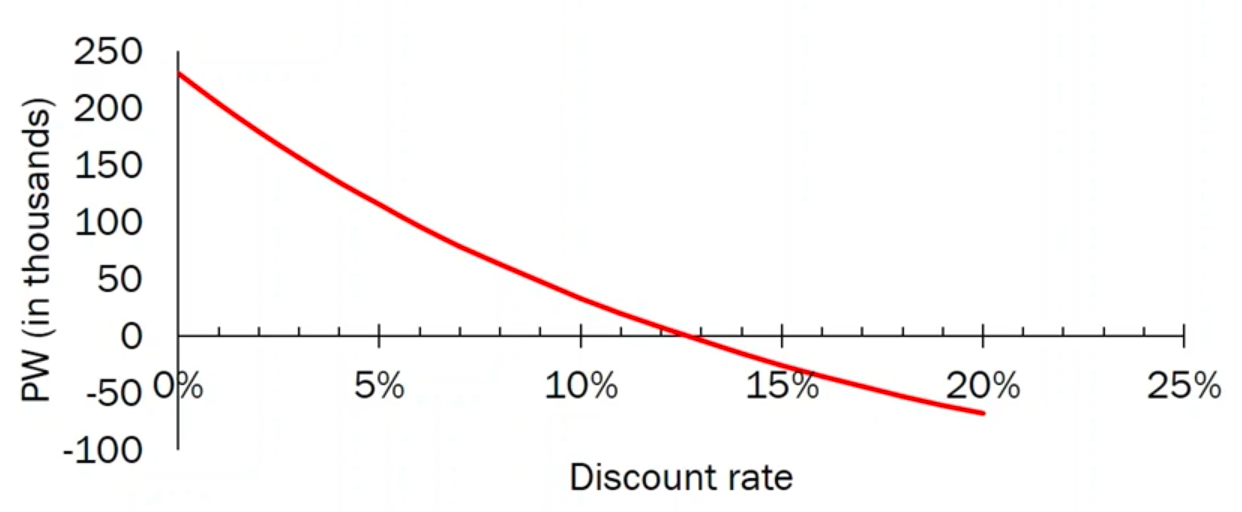
\includegraphics[width=0.5\textwidth]{LECTURE_6/IRR.png}
    \caption{PW vs. Discount Rate Graph for a Simple Project}
\end{figure}

\begin{proposition}
    [Evaluating Simple Projects with IRR]

    \textbf{Where the investment is simple} (i.e. all negative cash-flows precede positive cash-flows):
    \begin{itemize}
        \item If $IRR > MARR$, accept the project
        \item If $IRR < MARR$, reject the project
    \end{itemize}
\end{proposition}

\begin{proposition}
    [Limitations of IRR]
    When the investment is not simple, there will be two solutions to the equation that satisfies the PW = 0. In this case, it may not a good measure of the project's profitability.
\end{proposition}

\begin{figure}[H]
    \centering
    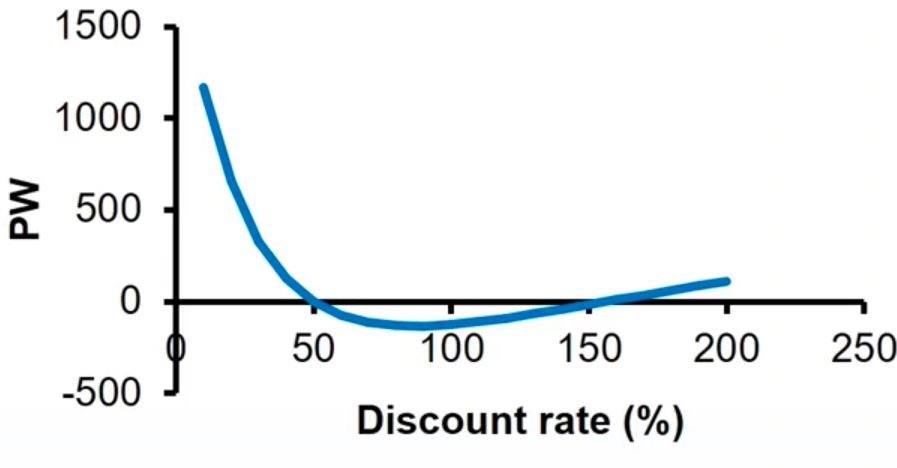
\includegraphics[width=0.5\textwidth]{LECTURE_6/not-simple.png}
    \caption{PW vs. Discount Rate Graph for a Complex Project}
\end{figure}

\section{Payback Period}


\begin{definition}
    [Payback Period]
    The payback period is the time it takes for the project to recover the initial investment.
\end{definition}

\begin{theorem}
    [Finding Payback Period]
    Using a cash-flow diagram, find the time it takes for the cumulative cash-flow to reach zero (not discounted).
\end{theorem}

\begin{theorem}
    [Discounted Payback Period]
    The discounted payback period is the time it takes for the \underline{discounted} cumulative cash-flow, the Present Worth, to reach zero.
\end{theorem}

\begin{proposition}
    [Evaluation of the Payback Period Method]
    \begin{itemize}
        \item Answers "When will I make my money back?"
        \item Easy to use/understand, \textbf{especially if the investment was not meant to make money}
        \item Not a sound method in Engineering Economics and against its principles
        \item[] \begin{itemize}
                  \item Ignores the cash-flows after the payback period, so it can overlook long-term investments
              \end{itemize}
    \end{itemize}
\end{proposition}

\section{Comparing Mutually Exclusive Projects Using IRR}

\begin{proposition}
    [IRR for Mutually Exclusive Projects]
    IRR can be misleading when comparing mutually exclusive projects. Take the following example:\\
    You can invest in the bank for a rate of return of $10\%$, or in the following projects:
    \begin{itemize}
        \item Lend your friend \$10 for a return of \$15 in 1 year (IRR = $50\%$)
        \item Lend your friend \$20 for a return of \$28 in 1 year (IRR = $40\%$)
    \end{itemize}
    The IRR method would suggest that you should lend your friend \$10 but consider that investing \$10 in your friend and \$10 in the bank would yield $10\cdot 1.1 + 10\cdot 1.5 = 26$ which is less than $\$20\cdot 1.4 = 28$, so you should invest in the second project. \\
    \textbf{Therefore, the IRR can mislead when the size of the investment is not considered.}
\end{proposition}
\begin{theorem}
    [Incremental IRR]
    This solves the problem of comparing mutually exclusive projects by comparing increments between two projects.\\
    \begin{itemize}
        \item Order alternatives in increasing order of first costs
        \item Start with the 'do nothing' alternative
        \item Calculate the IRR of the first alternative, if it is greater than the MARR, keep this as the best option so far
        \item Calculate the iterative IRR of the next alternative compared to the previous best option
        \item When comparing two alternatives, get the $\Delta FC$ (difference in first costs) and $\Delta A$ (difference in annual benefits) and solve for $PW =0$ to get the IRR
    \end{itemize}
\end{theorem}